\chapter{Amplificatori Operazionali e Retroazione}
\label{ch:opamp}

\section{Introduzione agli Op-Amp}

\begin{definizione}{Amplificatore Operazionale (Op-Amp)}
L'amplificatore operazionale (Op-Amp) è, essenzialmente, un amplificatore differenziale caratterizzato da specifiche ideali o quasi ideali. Nella sua modellizzazione teorica, esso possiede:
\begin{itemize}
    \item Un \textbf{elevatissimo guadagno di tensione differenziale}, denotato con $A_d \geq 100 \text{ dB}$ (ossia circa $10^5$): essenziale per le operazioni in reazione;
    \item Un'\textbf{elevata reiezione di modo comune} (CMRR), che lo rende insensibile ai disturbi condivisi su entrambi gli ingressi;
    \item Un'\textbf{impedenza d'ingresso estremamente alta} ($Z_{in} \sim 10^5 \div 10^{12}\,\Omega$), progettata in modo da assorbire correnti quasi nulle dai circuiti a monte, evitando di caricarli;
    \item Un'\textbf{impedenza di uscita molto bassa} ($Z_{out} \sim 10\,\Omega$), fondamentale per pilotare carichi di vario genere senza subire repentine cadute di tensione.
\end{itemize}
\end{definizione}

\begin{osservazione}{Struttura interna}
A livello di blocchi funzionali, un amplificatore operazionale è costituito da tre stadi principali in cascata:
\begin{itemize}
    \item Lo \textbf{stadio di ingresso} è un amplificatore differenziale, che provvede all'elevata impedenza d'ingresso e al rifiuto del modo comune.
    \item Lo \textbf{stadio di guadagno} fornisce il grosso dell'amplificazione di tensione del dispositivo; a questo stadio è associata una capacità di compensazione $C_c$, introdotta volontariamente per garantire la stabilità qualora il componente operi in retroazione.
    \item Lo \textbf{stadio di uscita} è tipicamente un emitter follower a simmetria complementare (push-pull in classe AB), capace di fornire una bassa impedenza di uscita e di pilotare carichi.
\end{itemize}
\end{osservazione}

\begin{figure}[H]
    \centering
    \begin{circuitikz}[node distance=1.4cm, >=stealth, thick]
        % Blocchi
        \node[draw, rounded corners, minimum width=2.5cm, minimum height=1.2cm, align=center]
            (diff) {ingresso\\differenziale};
        \node[draw, rounded corners, minimum width=2.5cm, minimum height=1.2cm, align=center,
            right=of diff]
            (gain) {stadio di\\guadagno};
        \node[draw, rounded corners, minimum width=2.5cm, minimum height=1.2cm, align=center,
            right=of gain]
            (ef) {emitter follower\\a simmetria\\complementare};

        % Frecce principali
        \draw[->] (diff) -- (gain) coordinate[pos=0.5] (mid1);
        \draw[->] (gain) -- (ef) coordinate[pos=0.5] (mid2);
        \draw[->] (ef.east) -- ++(1,0) node[right] {$V_{out}$};

        % Ingressi
        \draw[<-] (diff.west) ++(0, 0.3) -- ++(-1,0) node[left] {$V_+$};
        \draw[<-] (diff.west) ++(0,-0.3) -- ++(-1,0) node[left] {$V_-$};

        % Capacità di compensazione Cc
        \draw (mid1) to[short, *-] ++(0, 1.4) coordinate (c_left);
        \draw (mid2) to[short, *-] ++(0, 1.4) coordinate (c_right);
        \draw (c_left) to[C, l=$C_c$] (c_right);
        \node[above=0.6cm of c_right, anchor=south east, align=center, font=\footnotesize]
            {capacità di compensazione\\(stabilezza)};

        % GND sotto gain
        \draw (gain.south) -- ++(0,-0.4) node[ground] {};
    \end{circuitikz}
    \caption{Struttura interna a blocchi dell'amplificatore operazionale.}
    \label{fig:opamp_blocks}
\end{figure}

\subsection*{Simbolo circuitale e caratteristica}

\begin{figure}[H]
    \centering
    \begin{minipage}[c]{0.38\textwidth}
        \centering
        \begin{circuitikz}[american, transform shape]
            \draw (0,0) node[op amp] (opamp) {};
            \draw (opamp.-) node[left] {$V_-$};
            \draw (opamp.+) node[left] {$V_+$};
            \draw (opamp.out) to[short,-o] ++(0.3,0) node[right] {$V_{out}$};
            \draw (opamp.up)  -- ++(0,0.4) node[above] {$V_{CC}$};
            \draw (opamp.down) -- ++(0,-0.4) node[below] {$V_{EE}$};
        \end{circuitikz}
    \end{minipage}%
    \hfill
    \begin{minipage}[c]{0.55\textwidth}
        \centering
        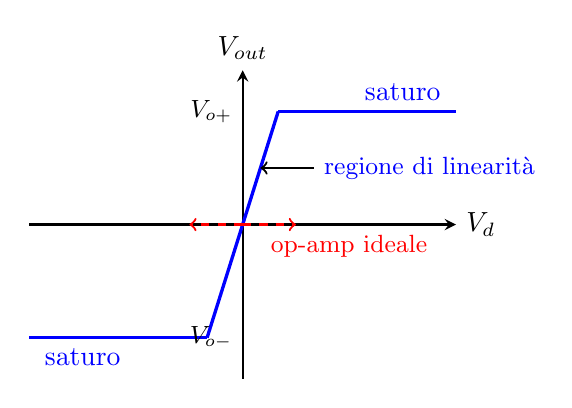
\begin{tikzpicture}
            \begin{axis}[
                width=7cm, height=5.5cm,
                xlabel={$V_d$},
                ylabel={$V_{out}$},
                xmin=-0.06, xmax=0.06,
                ymin=-1.5, ymax=1.5,
                xtick=\empty, ytick=\empty,
                axis lines=center,
                clip=false,
                thick,
                every axis x label/.style={at={(ticklabel* cs:1)},anchor=west},
                every axis y label/.style={at={(ticklabel* cs:1)},anchor=south},
            ]
                % Zona satura negativa
                \addplot[blue, very thick, domain=-0.06:-0.01] {-1.1} node[pos=0.3, below] {saturo};
                % Zona lineare
                \addplot[blue, very thick, domain=-0.01:0.01] {110*x};
                % Zona satura positiva
                \addplot[blue, very thick, domain=0.01:0.06] {1.1} node[pos=0.7, above] {saturo};

                % Etichette saturazione su asse y
                \node[left, font=\small] at (axis cs: 0, 1.1) {$V_{o+}$};
                \node[left, font=\small] at (axis cs: 0,-1.1) {$V_{o-}$};

                % Frecce Vd e opamp ideale
                \draw[->, red, dashed, thick] (axis cs:0,0) -- (axis cs:0.015,0);
                \draw[->, red, dashed, thick] (axis cs:0,0) -- (axis cs:-0.015,0);
                \node[below right, font=\small, text=red] at (axis cs: 0.005, 0) {op-amp ideale};
                
                \draw[<-] (axis cs: 0.005, 0.55) -- (axis cs: 0.02, 0.55) node[right, font=\small, text=blue] {regione di linearità};
            \end{axis}
        \end{tikzpicture}
    \end{minipage}
    \caption{Simbolo circuitale (sinistra) e caratteristica di trasferimento $V_{out}$ vs $V_d$ (destra).}
\end{figure}

\begin{definizione}{Funzionamento Lineare e Saturazione}
    In regione di funzionamento lineare, la tensione di uscita è direttamente proporzionale alla differenza di potenziale applicata ai morsetti di ingresso, tramite la relazione:
    \[ V_{out} = A_d (V_+ - V_-) = A_d V_d \]
    
    Tuttavia, data l'immensità del guadagno $A_d$, l'estensione della regione lineare sull'asse delle ascisse è limitata a una strettissima fascia di tensioni in ingresso, approssimativamente data da:
    \[ \Delta V_d \approx \frac{V_{CC} - V_{EE}}{A_d} \]
    Con alimentazioni di qualche decina di volt e $A_d \sim 10^5$ questa fascia è di circa $10^{-4}$\,V (qualche centinaio di microvolt; ancora meno per guadagni più alti), un valore paragonabile o \textbf{inferiore all'ampiezza del rumore e degli offset} presenti in un circuito reale. Al di fuori di questo ristretto intervallo, l'uscita del dispositivo satura immediatamente alle tensioni $V_{o+}$ o $V_{o-}$ (molto vicine alle alimentazioni).
\end{definizione}

Pertanto, affinché l'amplificatore operazionale possa essere utilizzato stabilmente in zona lineare come amplificatore di segnale (evitando che il solo rumore di fondo lo spinga in saturazione), è strettamente necessario ricorrere a una rete di \textbf{retroazione (feedback) negativa}: per creare una rete amplificatrice stabile dobbiamo inserire l'op-amp in un circuito che lo vincoli alla zona lineare, in modo che la retta di carico intersechi la curva dell'op-amp proprio nella sua regione di linearità.

\section{Configurazioni Fondamentali}

\subsection{Amplificatore Invertente}

\begin{osservazione}{Ingressi}
    \begin{itemize}
        \item Ingresso $+$ (non invertente): il segnale \textbf{non} viene invertito
        \item Ingresso $-$ (invertente): il segnale viene invertito
    \end{itemize}
\end{osservazione}

\begin{figure}[H]
    \centering
    \begin{circuitikz}[american, transform shape]
        \draw (0,0) node[op amp] (opamp) {};
        
        % Linee in ingresso
        \draw (opamp.-) -- ++(-1.2, 0) coordinate(in_node);
        \draw (opamp.+) -- ++(-1.2, 0) coordinate(pos_node);
        \draw (pos_node) node[ground] {};
        
        % Nodo nero esatto all'incrocio (in_node)
        \filldraw[black] (in_node) circle (1.5pt);
        
        % R1 e terminale Vs (con pallino vuoto)
        \draw (in_node) to[R, l=$R_1$] ++(-2, 0) coordinate(vs_node);
        \draw[fill=white, thick] (vs_node) circle (1.5pt) node[left, xshift=-0.1cm] {$V_S$};
        
        % Resistenza di Miller tratteggiata rossa tra i due ingressi (verticale)
        \draw[color=red, dashed] (in_node) to[R, color=red] (pos_node);
        
        % R2 e ramo di retroazione
        \draw (in_node) -- ++(0, 1.5) coordinate(fb_start);
        \draw (fb_start) to[R, l=$R_2$, name=R2] (fb_start -| opamp.out) coordinate(fb_end);
        \draw (fb_end) -- (opamp.out);
        
        % Croce rossa e asterisco cerchiato (Teorema di Miller)
        \draw[color=red, thick] ($(fb_start)!0.8!(fb_end)$) ++(-0.15,-0.15) -- ++(0.3,0.3);
        \draw[color=red, thick] ($(fb_start)!0.8!(fb_end)$) ++(-0.15,0.15) -- ++(0.3,-0.3);
        \node[color=red, circle, draw, inner sep=0.5pt, font=\small, thick, above=0.2cm of R2, xshift=1.2cm] {$\ast$};

        % Connessione in uscita
        \filldraw[black] (opamp.out) circle (1.5pt);
        \draw (opamp.out) -- ++(1, 0) coordinate(out_node);
        \draw[fill=white, thick] (out_node) circle (1.5pt) node[right, xshift=0.1cm] {$V_{out}$};
    \end{circuitikz}
    \caption{Configurazione dell'amplificatore invertente.}
\end{figure}

\begin{teorema}{Guadagno dell'Amplificatore Invertente}
Considerando le ipotesi ideali in cui $Z_{in} \gg R_1, R_2$ (dunque $Z_{in} \to \infty$, il che implica che nessuna corrente entra nei morsetti dell'operazionale) e $Z_{out} \ll R_1, R_2, R_L$ (dunque $Z_{out} \to 0$), possiamo determinare la tensione sul morsetto invertente valutando il partitore di retroazione.

Applicando la legge di Kirchhoff ai nodi per il terminale invertente, e ricordando che esso non assorbe corrente:
\[
    \frac{V_S - V_-}{R_1} = \frac{V_- - V_{out}}{R_2}
\]
Risolvendo per $V_-$, si ottiene l'espressione generale:
\[
    V_- = \frac{R_2}{R_1+R_2}\,V_S + \frac{R_1}{R_1+R_2}\,V_{out}
\]
Dato che il morsetto non invertente è a massa ($V_+ = 0$), in zona lineare l'uscita è legata al solo morsetto invertente tramite $V_{out} = -A_d V_-$. Sostituendo questa condizione, possiamo esprimere l'uscita in funzione dell'ingresso e descriverla come un fascio di rette in $V_S$:
\[
    V_{out} = \frac{(R_1+R_2)\,V_- - R_2 V_S}{R_1}, \qquad V_- = -\frac{V_{out}}{A_d}
\]
Esplicitando infine il rapporto di amplificazione ad anello chiuso $A_v = V_{out}/V_S$, il guadagno risulta:
\[
    \boxed{A_v = -\frac{R_2}{R_2 + (1+A_d)R_1}\,A_d}
\]
Questa complessa relazione presenta una notevole analogia formale con il guadagno di un BJT in configurazione common-emitter, governato dal parametro $\beta$:
\[
    A_v^{CE} = -\frac{R_C}{r_{BE}+(1+\beta)R_E}\,\beta
\]
Tuttavia, poiché il guadagno differenziale $A_d$ è tipicamente immenso ($A_d \sim 10^5$, molto superiore al $\beta \sim 10^2$ del BJT), il termine $(1+A_d)R_1$ domina nettamente il denominatore. Di conseguenza, la formula si semplifica notevolmente nell'approssimazione ideale e risulta intrinsecamente più precisa:
\[
    \boxed{A_v \approx -\frac{R_2}{R_1}}
\]

\begin{osservazione}{Perché usiamo il Teorema di Miller?}
    Il \textbf{Teorema di Miller} (introdotto nella \cref{sec:miller-bjt}; evidenziato in \textcolor{red}{rosso} nello schema) è uno strumento matematico fondamentale per l'analisi dei circuiti con retroazione.
    
    La sua applicazione ci permette di \textit{disaccoppiare} idealmente l'ingresso dall'uscita. In pratica, la resistenza fisica $R_2$, che connette direttamente i due stadi, viene matematicamente "spezzata" e sostituita da due resistenze separate, entrambe riferite a massa.
    
    Questo sdoppiamento chiarisce in modo lampante il comportamento del circuito:
    \begin{itemize}
        \item \textbf{Impedenza riflessa:} La frazione di $R_2$ che viene vista all'ingresso assume il valore $R_{M_{in}} = \frac{R_2}{1+A_d}$.
        \item \textbf{Effetto del guadagno:} Poiché il guadagno $A_d$ dell'amplificatore è immenso, il denominatore diventa grandissimo. Di conseguenza, il valore della resistenza equivalente $R_{M_{in}}$ crolla, risultando \textbf{vicinissima a zero}.
    \end{itemize}
    
    \vspace{0.5em}
    \textbf{Conclusione (Il Cortocircuito Virtuale):}\\
    Avere un'impedenza equivalente quasi nulla collegata all'ingresso fa sì che quel ramo si comporti, a tutti gli effetti, come un cortocircuito. 
    Questo meccanismo è il fondamento fisico e matematico che giustifica l'importante \textbf{principio del cortocircuito virtuale}: la forte retroazione abbatte l'impedenza e costringe il nodo invertente a portarsi esattamente allo stesso potenziale del nodo non invertente, pur non essendoci alcun collegamento reale tra di essi.
\end{osservazione}

\end{teorema}

\subsection{Amplificatore Non Invertente}
Questa configurazione è, da un punto di vista topologico, \textbf{analoga a quella dell'amplificatore invertente, ma scambiando il ruolo della terra e della sorgente} $V_S$.

\begin{figure}[H]
    \centering
    \begin{circuitikz}[american, transform shape]
        \draw (0,0) node[op amp, yscale=-1] (opamp) {};
        
        % Ingressi
        \draw (opamp.+) -- ++(-1.2, 0) coordinate(pos_node);
        \draw[fill=white, thick] (pos_node) circle (1.5pt) node[left, xshift=-0.1cm] {$V_S$};
        
        \draw (opamp.-) -- ++(-1.2, 0) coordinate(in_node);
        \filldraw[black] (in_node) circle (1.5pt);
        \draw (in_node) to[R, l=$R_1$] ++(-2, 0) node[ground]{};
        
        % Retroazione
        \draw (in_node) -- ++(0, -1.5) coordinate(fb_start);
        \draw (fb_start) to[R, l=$R_2$] (fb_start -| opamp.out) coordinate(fb_end);
        \draw (fb_end) -- (opamp.out);
        
        % Uscita
        \filldraw[black] (opamp.out) circle (1.5pt);
        \draw (opamp.out) -- ++(1, 0) coordinate(out_node);
        \draw[fill=white, thick] (out_node) circle (1.5pt) node[right, xshift=0.1cm] {$V_{out}$};
    \end{circuitikz}
    \caption{Configurazione dell'amplificatore non invertente.}
\end{figure}

\begin{teorema}{Guadagno dell'Amplificatore Non Invertente}
Il segnale da amplificare è applicato direttamente al morsetto non invertente ($V_+ = V_S$), mentre la rete di retroazione riporta una frazione del segnale d'uscita sul morsetto invertente.

La tensione al nodo $V_-$ è determinata dal partitore di tensione formato da $R_1$ ed $R_2$, per cui possiamo scrivere il sistema:
\[
    V_- = \frac{R_1}{R_1+R_2} V_{out} \quad \text{e} \quad V_+ = V_S
\]
Sapendo che la tensione differenziale è $V_d = V_+ - V_-$, possiamo esplicitare $V_{out}$ in funzione di $V_S$ e $V_d$:
\[
    \Rightarrow V_{out} = \frac{R_1+R_2}{R_1} (V_S - V_d)
\]
Considerando ora il funzionamento in \textbf{zona lineare}, l'amplificatore impone la relazione $V_{out} = A_d V_d$ (da cui $V_d = V_{out}/A_d$). Sostituendo questa espressione nell'equazione precedente e risolvendo per il rapporto $V_{out}/V_S$, si ottiene l'espressione esatta del guadagno $A_v$:
\[
    A_v = \frac{V_{out}}{V_S} = \frac{R_1+R_2}{R_2 + (1+A_d)R_1} A_d
\]
Essendo tipicamente il guadagno differenziale $A_d \gg 1$, il termine $(1+A_d)R_1$ al denominatore risulta preponderante, portando alla ben nota semplificazione per l'op-amp ideale:
\[
    \boxed{A_v \simeq 1 + \frac{R_2}{R_1} \ge 1} \quad \text{(poiché } A_d \gg 1\text{)}
\]
\end{teorema}

\begin{osservazione}{Analogia con il BJT}
    Come l'\textbf{emitter follower} (inseguitore di emettitore), l'amplificatore non invertente non inverte il segnale, ha impedenza d'ingresso molto alta e impedenza d'uscita molto bassa; in più permette un guadagno maggiore di 1 e ha prestazioni molto più vicine a quelle ideali rispetto a un singolo transistor. Il caso con guadagno unitario (voltage follower, sotto) è l'analogo diretto dell'emitter follower.
\end{osservazione}
\begin{osservazione}{Inseguitore di Tensione (Voltage Follower)}
    Se si rimuove la resistenza $R_1$ (equivalente a $R_1 \to \infty$) e si sostituisce $R_2$ con un cortocircuito ($R_2 = 0$), si ottiene la configurazione nota come \textbf{Voltage Follower}. In questo caso, il guadagno diventa esattamente $A_v = 1$. Questo circuito è di fondamentale importanza pratica in quanto possiede un'impedenza di ingresso altissima e una di uscita bassissima, fungendo da stadio separatore (buffer) ideale tra differenti sezioni di un sistema elettronico.
\end{osservazione}

\section{Principio del Corto Circuito Virtuale}
\label{sec:ccv}
I risultati precedenti per le configurazioni ideali si possono trovare in modo molto più immediato assumendo a priori che il guadagno ad anello aperto sia infinito ($A_d = \infty$).

Da un punto di vista grafico, la retta che descrive il comportamento dell'operazionale in zona lineare assume pendenza infinita, intersecando di fatto l'asse delle ordinate (coincidendo con un segmento verticale). Di conseguenza, se l'amplificatore sta operando in zona lineare e $A_d = \infty$, la differenza di potenziale in ingresso deve essere necessariamente nulla per restituire un'uscita finita:
\[
    \boxed{V_d = 0 \iff V_+ = V_-} \quad \text{nella zona di linearità}
\]

\begin{definizione}{Corto Circuito Virtuale (CCV)}
    In un amplificatore operazionale ideale ($A_d = \infty$), la tensione differenziale all'ingresso $V_d$ è nulla, per cui $V_+ = V_-$. La dicitura "virtuale" sottolinea che, sebbene i morsetti si trovino allo stesso potenziale, \textbf{nessuna corrente fluisce fra i due morsetti}, essendo l'impedenza di ingresso infinita.
\end{definizione}

\subsection{Esempio: Amplificatore Invertente (Modello di Miller)}
Rappresentiamo l'amplificatore invertente tramite un modello a due porte, applicando il \textbf{Teorema di Miller} per scomporre la resistenza di retroazione $R_2$.

\begin{figure}[H]
    \centering
    \begin{circuitikz}[american, transform shape]
        % Ingresso
        \draw (0,0) node[left] {$V_S$} to[short, o-] (0.5,0) to[R, l=$R_1$] (3,0) coordinate(in_node);
        \node[below] at (3, -0.2) {$V_1 = -V_d$};
        
        % Blocco due porte
        \draw (in_node) -- (4,0);
        \draw[thick] (4, -1) rectangle (6, 1);
        \node[align=center] at (5, 0) {Op-Amp};
        \draw (6,0) -- (7,0) coordinate(out_node);
        
        % Resistenze equivalenti di Miller (rosse)
        \draw[color=red, thick] (in_node) to[R, l_=$R'_2$, color=red] (3,-2.5) node[ground, color=black]{};
        \draw[color=red, thick] (out_node) to[R, l=$R''_2$, color=red] (7,-2.5) node[ground, color=black]{};
        
        % Uscita
        \node[below] at (7, -0.2) {$V_2 = V_{out}$};
        \draw (out_node) to[short, -o] (8,0) node[right] {$V_{out}$};
    \end{circuitikz}
    \caption{Rappresentazione a due porte dell'amplificatore invertente (Teorema di Miller).}
\end{figure}

Le resistenze equivalenti di Miller (evidenziate in rosso nello schema) assumono i seguenti valori:
\[
    \textcolor{red}{R'_2 = \frac{R_2}{1-K}} \quad \text{e} \quad \textcolor{red}{R''_2 = \frac{K}{K-1} R_2}, \qquad K = \frac{V_2}{V_1} = \frac{A_d V_d}{-V_d} = -A_d
\]
cioè
\[
    \textcolor{red}{R'_2 = \frac{R_2}{1+A_d}} \quad \text{e} \quad \textcolor{red}{R''_2 = \frac{A_d}{A_d+1} R_2 \simeq R_2}
\]
Queste espressioni valgono per qualunque valore di $A_d$ e descrivono il comportamento del circuito reale.

L'aspetto fondamentale emerge considerando il limite ideale dell'amplificatore, ovvero per un guadagno $A_d \to \infty$:
\[
    \lim_{A_d \to \infty} R'_2 = 0
\]
Poiché la resistenza $R'_2$ si annulla, il nodo di ingresso si trova di fatto connesso a massa tramite un'impedenza nulla. Questo meccanismo giustifica l'uso del termine \textbf{corto circuito virtuale} (o massa virtuale). Nei diagrammi circuitali a seguire, questo principio viene enfatizzato visivamente inserendo un \textbf{collegamento grigio} tra i morsetti invertente e non invertente dell'operazionale. Questa linea non rappresenta un vero filo conduttore, bensì il \emph{corto circuito virtuale} che vincola i due nodi ad assumere lo stesso potenziale ($V_+ = V_-$) senza assorbire corrente.

\subsection{Applicazioni del CCV}

\subsubsection*{1. Amplificatore invertente}
\begin{figure}[H]
    \centering
    \begin{circuitikz}[american, transform shape]
        \draw (0,0) node[op amp] (opamp) {};
        \draw[gray!50, line width=2pt] (opamp.+) -- (opamp.-);
        \draw (opamp.+) to[short] ++(0,-0.5) node[ground] {};
        \draw (opamp.-) to[short, *-] ++(-0.5, 0) coordinate(in_node);
        \draw (in_node) to[R, l=$R_1$, -o] ++(-2, 0) node[left] {$V_S$};
        \draw (in_node) -- ++(0, 1.2) coordinate(fb_start);
        \draw (fb_start) to[R, l=$R_2$] (fb_start -| opamp.out) coordinate(fb_end);
        \draw (opamp.out) to[short, *-] (fb_end);
        \draw (opamp.out) to[short, -o] ++(0.5, 0) node[right] {$V_{out}$};
    \end{circuitikz}
    \caption{Applicazione: Amplificatore invertente.}
\end{figure}
Ponendo a massa il terminale non invertente, si ha $V_+ = 0$. Applicando la sovrapposizione degli effetti al nodo invertente e sfruttando la condizione $V_+ = V_-$, otteniamo:
\[ 0 = V_+ = V_- = \frac{R_1}{R_1+R_2} V_{out} + \frac{R_2}{R_1+R_2} V_S \implies A_v = -\frac{R_2}{R_1} \]

\subsubsection*{2. Amplificatore non invertente}
\begin{figure}[H]
    \centering
    \begin{circuitikz}[american, transform shape]
        \draw (0,0) node[op amp] (opamp) {};
        \draw[gray!50, line width=2pt] (opamp.+) -- (opamp.-);
        \draw (opamp.+) to[short, -o] ++(-1, 0) node[left] {$V_S$};
        \draw (opamp.-) to[short, *-] ++(-0.5, 0) coordinate(in_node);
        \draw (in_node) to[R, l=$R_1$] ++(-1.5, 0) to[short] ++(0,-0.5) node[ground] {};
        \draw (in_node) -- ++(0, 1.2) coordinate(fb_start);
        \draw (fb_start) to[R, l=$R_2$] (fb_start -| opamp.out) coordinate(fb_end);
        \draw (opamp.out) to[short, *-] (fb_end);
        \draw (opamp.out) to[short, -o] ++(0.5, 0) node[right] {$V_{out}$};
    \end{circuitikz}
    \caption{Applicazione: Amplificatore non invertente.}
\end{figure}
Applicando il segnale al morsetto non invertente, si ha $V_+ = V_S$. Sfruttando la condizione del CCV ($V_+ = V_-$) e valutando il partitore di tensione sul ramo di retroazione, otteniamo:
\[ V_S = V_+ = V_- = \frac{R_1}{R_1+R_2} V_{out} \implies A_v = 1 + \frac{R_2}{R_1} \]

\subsubsection*{3. Circuito sommatore invertente}
\begin{figure}[H]
    \centering
    \begin{circuitikz}[american, transform shape]
        \draw (0,0) node[op amp] (opamp) {};
        \draw[gray!50, line width=2pt] (opamp.+) -- (opamp.-);
        \draw (opamp.+) to[short] ++(0,-0.5) node[ground] {};
        \draw (opamp.-) to[short, *-] ++(-0.5, 0) coordinate(in_node);
        \draw (in_node) -- ++(0, 1.2) coordinate(fb_start);
        \draw (fb_start) to[R, l=$R$] (fb_start -| opamp.out) coordinate(fb_end);
        \draw (opamp.out) to[short, *-] (fb_end);
        \draw (in_node) -- ++(-0.5, 0) coordinate(split_node);
        \draw (split_node) to[short, *-] ++(0, 0.5) to[R, l=$R_1$, -o] ++(-1.5, 0) node[left] {$V_1$};
        \draw (split_node) to[short, *-] ++(0, -0.5) to[R, l=$R_2$, -o] ++(-1.5, 0) node[left] {$V_2$};
        \draw (opamp.out) to[short, -o] ++(0.5, 0) node[right] {$V_{out}$};
    \end{circuitikz}
    \caption{Configurazione del sommatore invertente.}
\end{figure}
Sfruttando la proprietà della massa virtuale ($V_- = 0$) e applicando la sovrapposizione degli effetti, possiamo esprimere l'uscita come somma pesata degli ingressi ($V_{out} = A_1 V_1 + A_2 V_2$):
\[ V_{out} = A_1 V_1 + A_2 V_2 \implies A_1 = -\frac{R}{R_1} \quad ; \quad A_2 = -\frac{R}{R_2} \]

\subsubsection*{4. Circuito sommatore non invertente}
\begin{figure}[H]
    \centering
    \begin{circuitikz}[american, transform shape]
        \draw (0,0) node[op amp] (opamp) {};
        \draw[gray!50, line width=2pt] (opamp.+) -- (opamp.-);
        
        % inverting terminal (top)
        \draw (opamp.-) to[short, *-] ++(-0.5, 0) coordinate(in_neg);
        \draw (in_neg) -- ++(0, 0.8) coordinate(R_level);
        \draw (R_level) to[R, l=$R$] ++(-2, 0) node[ground]{};
        \draw (in_neg) -- ++(0, 2) coordinate(fb_start);
        \draw (fb_start) to[R, l=$R'$] (fb_start -| opamp.out) coordinate(fb_end);
        \draw (opamp.out) to[short, *-] (fb_end);
        
        % non inverting terminal (bottom)
        \draw (opamp.+) to[short] ++(-0.5, 0) coordinate(in_pos);
        \draw (in_pos) -- ++(0, -0.5) coordinate(split_pos);
        \draw (split_pos) to[short, *-] ++(0, 0.5) to[R, l=$R_1$, -o] ++(-2, 0) node[left] {$V_1$};
        \draw (split_pos) to[short, *-] ++(0, -1.0) to[R, l=$R_2$, -o] ++(-2, 0) node[left] {$V_2$};
        
        \draw (opamp.out) to[short, -o] ++(0.5, 0) node[right] {$V_{out}$};
    \end{circuitikz}
    \caption{Configurazione del sommatore non invertente.}
\end{figure}
La tensione al nodo non invertente è fornita dal principio di sovrapposizione degli effetti sui generatori d'ingresso, dopodiché il segnale subisce il guadagno tipico dell'amplificatore non invertente. I guadagni per i singoli canali risultano:
\[ A_1 = \left( 1 + \frac{R'}{R} \right) \frac{R_2}{R_1+R_2} \quad ; \quad A_2 = \left( 1 + \frac{R'}{R} \right) \frac{R_1}{R_1+R_2} \]

\subsubsection*{5. Circuito sottrattore}
\begin{figure}[H]
    \centering
    \begin{circuitikz}[american, transform shape]
        \draw (0,0) node[op amp] (opamp) {};
        \draw[gray!50, line width=2pt] (opamp.+) -- (opamp.-);
        
        % inverting (top)
        \draw (opamp.-) to[short, *-] ++(-0.5, 0) coordinate(in_neg);
        \draw (in_neg) to[R, l=$R_1$, -o] ++(-1.5, 0) node[left] {$V_1$};
        \draw (in_neg) -- ++(0, 1.2) coordinate(fb_start);
        \draw (fb_start) to[R, l=$R_2$] (fb_start -| opamp.out) coordinate(fb_end);
        \draw (opamp.out) to[short, *-] (fb_end);
        
        % non inverting (bottom)
        \draw (opamp.+) to[short, *-] ++(-0.5, 0) coordinate(in_pos);
        \draw (in_pos) to[R, l=$R_3$, -o] ++(-1.5, 0) node[left] {$V_2$};
        \draw (in_pos) to[R, l=$R_4$] ++(0, -1.5) node[ground]{};
        
        \draw (opamp.out) to[short, -o] ++(0.5, 0) node[right] {$V_{out}$};
    \end{circuitikz}
    \caption{Configurazione dell'amplificatore differenziale o sottrattore.}
\end{figure}
Applicando il principio di sovrapposizione degli effetti tra i due ingressi per determinare i rispettivi guadagni, si ottiene:
\[ A_1 = -\frac{R_2}{R_1} \quad ; \quad A_2 = \frac{R_4/(R_3+R_4)}{R_1/(R_1+R_2)} \]

\vspace{0.5em}
\noindent\textcolor{red}{*} \textbf{Caso particolare:} Se l'uscita desiderata è $V_{out} = G(V_2 - V_1)$, otteniamo un \textbf{amplificatore differenziale a guadagno controllato} $G$ (da non confondere con il guadagno ad anello aperto $A_d$ dell'operazionale). In questa condizione i due guadagni devono essere uguali in modulo:
\[
    \colorbox{red!20}{$\displaystyle G = -A_1 = A_2 \implies \frac{R_3}{R_4} = \frac{R_1}{R_2} \implies G = \frac{R_2}{R_1}$}
\]
In questo modo l'uscita dipende solo dalla differenza dei due ingressi e non dal loro valor medio (reiezione del modo comune).

\section{Filtri attivi e circuiti lineari}

Fino ad ora abbiamo considerato circuiti amplificatori basati esclusivamente su resistenze, il cui comportamento è indipendente dalla frequenza del segnale in ingresso. Introducendo componenti reattivi, come i condensatori, all'interno della rete di retroazione o in ingresso, possiamo progettare \textbf{filtri attivi} e \textbf{circuiti lineari dinamici} (in grado di eseguire operazioni matematiche come l'integrazione o la derivazione di un segnale nel tempo).

\begin{definizione}{Funzione di Trasferimento Generalizzata}
    Considerando di operare nella regione lineare dell'amplificatore operazionale (assumendolo ideale), possiamo applicare il \textbf{Principio del Corto Circuito Virtuale}. Generalizziamo quindi la configurazione invertente sostituendo le resistenze con impedenze generiche $Z_1$ e $Z_2$.
    
    Per l'ipotesi di corto circuito virtuale, il morsetto invertente si trova a massa virtuale ($V_- \approx V_+ = 0\text{ V}$) e non assorbe corrente ($I_- = 0$). Applicando la legge di Kirchhoff per le correnti al nodo invertente, la corrente che attraversa $Z_1$ deve necessariamente attraversare anche $Z_2$:
    \[ I_{Z1} = \frac{V_S - 0}{Z_1} \quad ; \quad I_{Z2} = \frac{0 - V_{out}}{Z_2} \implies I_{Z1} = I_{Z2} \implies \frac{V_S}{Z_1} = -\frac{V_{out}}{Z_2} \]
    Pertanto, la funzione di trasferimento generalizzata (o guadagno in tensione in funzione della frequenza) diventa:
    \[ A_V(j\omega) = \frac{V_{out}}{V_S} = -\frac{Z_2(j\omega)}{Z_1(j\omega)} \]
    Questa espressione è fondamentale poiché permette di modellare la risposta in frequenza del circuito semplicemente scegliendo opportunamente $Z_1$ e $Z_2$.
\end{definizione}

\begin{figure}[H]
    \centering
    \begin{circuitikz}[american, transform shape]
        \draw (0,0) node[op amp] (opamp) {};
        \draw (opamp.+) node[ground] {};
        \draw (opamp.-) to[short, *-] ++(-0.5, 0) coordinate(in_node);
        \draw (in_node) to[generic, l=$Z_1$] ++(-2, 0) node[left] {$V_S$};
        \draw (in_node) -- (in_node |- 0, 1.5) coordinate(fb_start);
        \draw (fb_start) to[generic, l=$Z_2$] (fb_start -| opamp.out) coordinate(fb_end);
        \draw (opamp.out) to[short, *-] (fb_end);
        \draw (opamp.out) to[short, -o] ++(0.5, 0) node[right] {$V_{out}$};
    \end{circuitikz}
    \caption{Configurazione invertente generalizzata per filtri attivi.}
\end{figure}

\subsubsection*{Caso 1: L'Integratore}

\textbf{1. Integratore Ideale ($Z_1 = R$, $Z_2 = \frac{1}{j\omega C}$)} \\
Se utilizziamo una resistenza in ingresso e un condensatore in retroazione, otteniamo un circuito in grado di integrare il segnale nel tempo.

\begin{figure}[H]
    \centering
    \begin{circuitikz}[american, transform shape]
        \draw (0,0) node[op amp] (opamp) {};
        \draw (opamp.+) node[ground] {};
        \draw (opamp.-) to[short, *-] ++(-0.5, 0) coordinate(in_node);
        \draw (in_node) to[R, l=$R$] ++(-2, 0) node[left] {$V_S$};
        \draw (in_node) -- (in_node |- 0, 1.5) coordinate(fb_start);
        \draw (fb_start) to[C, l=$C$] (fb_start -| opamp.out) coordinate(fb_end);
        \draw (opamp.out) to[short, *-] (fb_end);
        \draw (opamp.out) to[short, -o] ++(0.5, 0) node[right] {$V_{out}$};
    \end{circuitikz}
    \caption{Configurazione dell'integratore ideale.}
\end{figure}

\begin{itemize}[label=$\cdot$, leftmargin=*]
    \item \textbf{Analisi nel dominio della frequenza:} Sostituendo le espressioni delle impedenze nella formula generalizzata, otteniamo un guadagno inversamente proporzionale alla frequenza:
    \[ A_V(\omega) = - \frac{1/(j \omega C)}{R} = - \frac{1}{j \omega R C} \]
    \item \textbf{Analisi nel dominio del tempo:} Dal corto circuito virtuale, la corrente in ingresso è unicamente $i(t) = \frac{V_S(t)}{R}$. Tutta questa corrente fluisce nel condensatore, la cui tensione ai capi è $V_C(t) = \frac{1}{C} \int_0^t i(t') dt'$. Poiché $V_{out}(t) = - V_C(t)$, l'uscita è proporzionale all'integrale del segnale d'ingresso:
    \[ V_{out}(t) = - \frac{1}{RC} \int_0^t V_S(t') dt' + V_{out}(0) \]
\end{itemize}

\begin{osservazione}{Problema di stabilità (limiti dell'integratore ideale)}
    A frequenza nulla ($\omega \to 0$, ovvero per segnali continui o DC), l'impedenza del condensatore tende all'infinito ($Z_2 \to \infty$), comportandosi come un circuito aperto. In questa condizione il guadagno ad anello chiuso $A_V \to \infty$. Questo significa che qualsiasi pur minima tensione continua in ingresso (inclusa la naturale tensione di offset dell'amplificatore) verrà integrata nel tempo fino a portare inevitabilmente l'uscita in \textbf{saturazione} (ossia al valore massimo consentito dalle tensioni di alimentazione).
\end{osservazione}

\vspace{0.2cm}
\textbf{2. Integratore Reale (Filtro Passa-Basso)} \\
Per evitare la saturazione in DC, si introduce una resistenza di scarica $R_2$ in parallelo al condensatore $C$. In questo modo, a bassa frequenza la retroazione è garantita da $R_2$.

\begin{figure}[H]
    \centering
    \begin{circuitikz}[american, transform shape]
        \draw (0,0) node[op amp] (opamp) {};
        \draw (opamp.+) node[ground] {};
        \draw (opamp.-) to[short, *-] ++(-0.5, 0) coordinate(in_node);
        \draw (in_node) to[R, l=$R_1$] ++(-2, 0) node[left] {$V_S$};
        
        \draw (in_node) -- (in_node |- 0, 1.5) coordinate(fb_start1);
        \draw (fb_start1) to[C, l=$C$] (fb_start1 -| opamp.out) coordinate(fb_end1);
        \draw (opamp.out) to[short, *-] (fb_end1);
        
        \draw (fb_start1) -- (in_node |- 0, 2.8) coordinate(fb_start2);
        \draw (fb_start2) to[R, color=red, l=$R_2$] (fb_start2 -| opamp.out) coordinate(fb_end2);
        \draw (fb_end1) -- (fb_end2);
        
        \draw (opamp.out) to[short, -o] ++(0.5, 0) node[right] {$V_{out}$};
    \end{circuitikz}
\caption{Configurazione dell'integratore reale.}
\end{figure}

L'impedenza di retroazione diventa $Z_2 = R_2 \parallel \frac{1}{j\omega C} = \frac{R_2}{1 + j\omega R_2 C}$. La nuova funzione di trasferimento è:
\[ A_V(\omega) = - \frac{Z_2}{Z_1} = - \frac{R_2}{R_1} \frac{1}{1 + j \omega R_2 C} \]
Si tratta di un tipico \textcolor{red}{\textbf{filtro passa-basso}}. 
\begin{itemize}[label=$\cdot$, leftmargin=*]
    \item Il \textbf{guadagno in continua} ($\omega \to 0$) è ora limitato al valore costante $A_{VMAX} = -\frac{R_2}{R_1}$, risolvendo il problema della saturazione.
    \item La \textbf{frequenza di taglio} superiore, a cui il guadagno scende di -3dB, vale $\textcolor{red}{f_L = \frac{1}{2 \pi R_2 C}}$. Oltre questa frequenza, il circuito si comporta come un buon integratore.
\end{itemize}


\subsubsection*{Caso 2: Il Derivatore}

\textbf{1. Derivatore Ideale ($Z_1 = \frac{1}{j\omega C}$, $Z_2 = R$)} \\
Scambiando i componenti rispetto all'integratore, si ottiene un derivatore.

\begin{figure}[H]
    \centering
    \begin{circuitikz}[american, transform shape]
        \draw (0,0) node[op amp] (opamp) {};
        \draw (opamp.+) node[ground] {};
        \draw (opamp.-) to[short, *-] ++(-0.5, 0) coordinate(in_node);
        \draw (in_node) to[C, l=$C$] ++(-2, 0) node[left] {$V_S$};
        \draw (in_node) -- (in_node |- 0, 1.5) coordinate(fb_start);
        \draw (fb_start) to[R, l=$R$] (fb_start -| opamp.out) coordinate(fb_end);
        \draw (opamp.out) to[short, *-] (fb_end);
        \draw (opamp.out) to[short, -o] ++(0.5, 0) node[right] {$V_{out}$};
    \end{circuitikz}
    \caption{Configurazione del derivatore ideale.}
\end{figure}

\begin{itemize}[label=$\cdot$, leftmargin=*]
    \item \textbf{Analisi nel dominio della frequenza:} Il guadagno è direttamente proporzionale alla frequenza:
    \[ A_V(\omega) = - \frac{R}{1/(j \omega C)} = - j \omega R C \]
    \item \textbf{Analisi nel dominio del tempo:} La corrente che attraversa il condensatore in ingresso è determinata dalle variazioni del segnale: $i(t) = C \frac{d V_S(t)}{dt}$. A causa del corto circuito virtuale, questa stessa corrente fluisce attraverso la resistenza di retroazione, per cui la tensione in uscita risulta essere la derivata dell'ingresso:
    \[ V_{out}(t) = - R i(t) = - R C \frac{d V_S(t)}{dt} \]
\end{itemize}

\begin{osservazione}{Problema di instabilità (limiti del derivatore ideale)}
    Alle alte frequenze ($\omega \to \infty$), l'impedenza del condensatore di ingresso $Z_1 \to 0$. Di conseguenza, il guadagno del derivatore tende all'infinito ($A_V \to \infty$). Questo rende il circuito estremamente sensibile al \textbf{rumore ad alta frequenza}, che verrà inevitabilmente amplificato fino a causare instabilità o saturazione.
\end{osservazione}

\vspace{0.2cm}
\textbf{2. Derivatore Reale (Filtro Passa-Alto)} \\
Per limitare il guadagno alle alte frequenze, si inserisce una resistenza $R_1$ in serie al condensatore di ingresso $C$.

\begin{figure}[H]
    \centering
    \begin{circuitikz}[american, transform shape]
        \draw (0,0) node[op amp] (opamp) {};
        \draw (opamp.+) node[ground] {};
        \draw (opamp.-) to[short, *-] ++(-0.5, 0) coordinate(in_node);
        \draw (in_node) to[C, l=$C$] ++(-1.5, 0) to[R, color=red, l=$R_1$] ++(-1.5, 0) node[left] {$V_S$};
        \draw (in_node) -- (in_node |- 0, 1.5) coordinate(fb_start);
        \draw (fb_start) to[R, l=$R_2$] (fb_start -| opamp.out) coordinate(fb_end);
        \draw (opamp.out) to[short, *-] (fb_end);
        \draw (opamp.out) to[short, -o] ++(0.5, 0) node[right] {$V_{out}$};
    \end{circuitikz}
    \caption{Configurazione del derivatore reale.}
\end{figure}

La nuova impedenza di ingresso diventa $Z_1 = R_1 + \frac{1}{j\omega C} = \frac{1 + j\omega R_1 C}{j\omega C}$. L'espressione per il guadagno diventa:
\[ A_V(\omega) = - \frac{R_2}{R_1 + \frac{1}{j\omega C}} = - \frac{j \omega R_2 C}{1 + j \omega R_1 C} \]
Questo circuito implementa un \textcolor{red}{\textbf{filtro passa-alto}}.
\begin{itemize}[label=$\cdot$, leftmargin=*]
    \item Il \textbf{guadagno ad alte frequenze} ($\omega \to \infty$) viene limitato al rapporto delle due resistenze $A_{VMAX} = -\frac{R_2}{R_1}$, proteggendo il circuito dal rumore.
    \item La \textbf{frequenza di taglio} vale $\textcolor{red}{f_H = \frac{1}{2 \pi R_1 C}}$. A frequenze notevolmente inferiori a $f_H$, il circuito si comporta come un buon derivatore.
\end{itemize}

\begin{osservazione}{Considerazioni sul Prodotto Guadagno-Banda (GBW)}
    Nei dispositivi reali il prodotto tra guadagno e banda dell'operazionale è costante (GBW, vedi la sezione seguente): con un guadagno ad anello chiuso $|A_{VMAX}| = \frac{R_2}{R_1}$, l'operazionale funziona correttamente solo fino a circa $f_{\max} \simeq \frac{\text{GBW}}{|A_{VMAX}|}$. Di conseguenza, un \textbf{guadagno massimo elevato} restringe la banda utile del filtro:
    \begin{itemize}[label=$\cdot$, leftmargin=*]
        \item passa-basso (integratore reale): la zona in cui il circuito integra correttamente, cioè fra $f_L$ e $f_{\max}$, si riduce;
        \item passa-alto (derivatore reale): la banda passante, che va da $f_H$ a $f_{\max}$, si riduce, perché $f_{\max}$ diminuisce all'aumentare del guadagno.
    \end{itemize}
\end{osservazione}

\section{Caratteristiche reali degli Op-Amp}

Un amplificatore operazionale reale si discosta dal modello ideale a causa di alcuni limiti fisici e tecnologici. I principali effetti sono tre:

\begin{enumerate}[label=\textbf{\arabic*.}, leftmargin=*, itemsep=0.4cm, topsep=0.3cm]

    \item \textbf{Capacità parassita in parallelo allo stadio di guadagno $\Rightarrow$ effetto = filtro passa-basso ($f_L$)}

    Per il teorema di Miller, il guadagno differenziale diventa dipendente dalla frequenza. Considerando l'ampiezza (modulo), si ha:
    \[ A_d(\omega) = \frac{A_0}{\sqrt{1 + \left(\frac{\omega}{\omega_0}\right)^2}} \]
    dove $A_0$ è il guadagno in continua (o a centro-banda).

    \begin{osservazione}{Esempio: amplificatore non invertente}
        Nel circuito non invertente la tensione al morsetto invertente è $V_- = \frac{R_1}{R_1 + R_2} V_{out} \equiv \beta V_{out}$ e $V_+ = V_S$.
        Da cui si ottiene $V_{out} = \frac{A_d}{1 + \beta A_d} V_S$. Questo comporta due conseguenze fondamentali:
        \begin{itemize}[label=$\Rightarrow$, leftmargin=*, noitemsep, topsep=0.1cm, parsep=0pt]
            \item \textbf{Guadagno massimo:} $A_M = \frac{A_0}{1 + \beta A_0} < A_0 = \text{guadagno di centro-banda}$
            \item \textbf{Frequenza di taglio:} $f_L = f_0 (1 + \beta A_0) > f_0 = \text{frequenza del filtro}$
        \end{itemize}
        \vspace{0.2cm}
        \textcolor{noteteal}{\textbf{$\Rightarrow$ invarianza del prodotto GBW:}} 
        \[ GBW = A_M \cdot f_L = A_0 \cdot f_0 = \text{invariante} \]
    \end{osservazione}

    \item \textbf{Capacità parassita + corrente limitata in uscita $\Rightarrow$ effetto = slew-rate}

    La corrente limitata in uscita ($I_C < \infty$) combinata alla capacità parassita impone che:
    \[ C \frac{d V_C}{dt} = I_C < \infty \implies \frac{d V_C}{dt} < \infty \]
    La tensione ai capi della capacità dello stadio di guadagno non può quindi variare istantaneamente, e questo limite si trasmette agli stadi successivi: $V_{out}$ può variare solo con una pendenza finita. La massima pendenza ottenibile si chiama \textbf{slew-rate} (tipicamente espressa in V/$\mu$s):
    \[ SR = \max \left( \frac{d V_{out}}{dt} \right) \]

    \begin{figure}[H]
        \centering
        \begin{tikzpicture}[scale=1.5]
            % Segnale ideale (quadrato, grigio, tratto spesso)
            \draw[line width=3.5pt, color=gray!70] 
                (0.2,0) -- (0.8,0) -- (0.8,1.8) -- (2.8,1.8) -- (2.8,0) -- (3.4,0);
            
            % Segnale reale con slew-rate (trapezio, verde/noteteal, tratto spesso)
            \draw[line width=3.5pt, color=noteteal, opacity=0.85] 
                (0,0) -- (0.8,0) -- (1.5,1.8) -- (2.8,1.8) -- (3.5,0) -- (3.8,0);
        \end{tikzpicture}
        \caption{Effetto dello slew-rate: a fronte di una variazione istantanea a gradino (in grigio), l'uscita (in verde) non potendo variare istantaneamente si adegua con una pendenza limitata, assumendo una caratteristica forma trapezoidale.}
    \end{figure}

    \item \textbf{Asimmetria nei transistor dello stadio di ingresso $\Rightarrow$ effetto = Offset di $\sim 10^{-1} \text{ mV}$ su $V_d$}

    In un Op-Amp ideale, applicando $0\text{ V}$ ad entrambi i morsetti ($V_d = 0$), ci si aspetta che l'uscita sia esattamente nulla. Nella realtà, il primo stadio interno di amplificazione è costituito da una coppia differenziale di transistor. Essendo fisicamente impossibile costruire due componenti in silicio identici al 100\%, ci sarà sempre una microscopica asimmetria costruttiva.

    Tale asimmetria fa sì che i due rami del circuito conducano correnti lievemente diverse anche a riposo. L'amplificatore interpreta questo squilibrio interno come se ci fosse un segnale, finendo per amplificarlo e producendo in uscita una tensione diversa da zero (talvolta sufficiente a mandare il dispositivo in saturazione).

    Per modellare questo difetto, si immagina di porre in serie ad uno dei morsetti di un Op-Amp ideale un piccolo generatore di tensione continuo fittizio (una sorta di "batteria"). Questo errore è definito \textbf{Tensione di Offset} ($V_{os}$) ed ha tipicamente un valore di circa $10^{-1}\text{ mV}$. A livello pratico, $V_{os}$ rappresenta l'esatta differenza di potenziale che si dovrebbe applicare volontariamente tra gli ingressi per riuscire a compensare lo squilibrio e forzare l'uscita a $0\text{ V}$.

\end{enumerate}

\section{Altri amplificatori con Op-Amp}

\subsubsection*{6. Amplificatore Invertente 2.0 (con Rete a T)}
\begin{figure}[H]
    \centering
    \begin{circuitikz}[american, transform shape]
        \draw (0,0) node[op amp] (opamp) {};
        \draw (opamp.+) -- ++(0,-0.5) node[ground] {};
        
        \draw (opamp.-) to[short, *-] ++(-1.5, 0) coordinate(in_node);
        \draw (in_node) ++(-2, 0) node[left] {$V_S$} to[R, l=$R$, o-] (in_node);
        
        % T-network
        \draw (in_node) -- ++(0, 2) coordinate(fb_start);
        \draw (fb_start) to[R, l=$R$] ++(3.5, 0) coordinate(t_center);
        \draw (t_center) node[above=0.1cm] {\textbf{a}};
        \draw (t_center) to[R, l=$R$] ++(2.5, 0) coordinate(fb_end);
        \draw (fb_end) |- (opamp.out);
        \draw (opamp.out) to[short, *-o] ++(1, 0) node[right] {$V_{out}$};
        
        % R' to ground from t_center
        \draw (t_center) to[R, l=$R'$] ++(0, -1.5) node[ground] {};
        
        % Gray arrows hugging the wires
        \draw[->, >=stealth, gray, thick, rounded corners=3mm] ([xshift=-0.2cm, yshift=0.2cm]in_node) |- ([xshift=1.0cm, yshift=0.2cm]fb_start) node[above, text=gray] {$I_S$};
        \draw[->, >=stealth, gray, thick] ([xshift=-0.4cm, yshift=-0.2cm]t_center) -- ([xshift=-0.4cm, yshift=-1.2cm]t_center) node[left, text=gray] {$I'$};
        \draw[->, >=stealth, gray, thick, rounded corners=3mm] ([xshift=1.0cm, yshift=0.2cm]t_center) -| ([xshift=0.3cm, yshift=-0.8cm]fb_end) node[right, text=gray] {$I$};
    \end{circuitikz}
    \caption{Amplificatore invertente con retroazione a rete a T.}
\end{figure}

\begin{teorema}{Analisi Invertente con Rete a T}
    Risolvendo la maglia di retroazione considerando la massa virtuale ($V_- = 0$), la corrente di ingresso è $I_S = V_S/R$. Questa scorre interamente verso il nodo \textbf{a}, portandolo a un potenziale $V_a = -V_S$. Al nodo \textbf{a} la corrente $I_S$ si divide fra $R'$ (verso massa) e la resistenza $R$ verso l'uscita:
    \[ I' = \frac{V_a}{R'} = -\frac{V_S}{R'}, \qquad I = I_S - I' = \frac{V_S}{R} + \frac{V_S}{R'} \]
    \[ V_{out} = V_a - R\,I = -V_S - V_S - \frac{R}{R'}V_S \implies A_V = - \left( 2 + \frac{R}{R'} \right) \]
    
    \noindent \textbf{Differenze con l'amplificatore invertente base (circuito 1):}
    \begin{itemize}[label=$\ast$, leftmargin=*, itemsep=0.1cm, topsep=0.1cm]
        \item \textbf{Guadagno minimo:} In questa configurazione $|A_V| \geq 2$, mentre nel circuito base può essere anche $|A_V| < 1$.
        \item \textbf{Impedenza di ingresso:} in entrambi i casi è pari alla resistenza d'ingresso ($Z_{in} = R$ qui, $Z_{in} = R_1$ nel circuito base). Nel circuito base, però, per avere un'impedenza d'ingresso alta \emph{e} un guadagno alto servirebbe una $R_2$ enorme; con la rete a T il guadagno si alza riducendo $R'$, senza usare resistenze di valore elevato.
        \item \textbf{Proporzionalità:} Aumentando $R$, il modulo del guadagno $A_V$ aumenta ($A_V(R \uparrow) \uparrow$); nel circuito base, aumentando la resistenza di ingresso $R_1$, il guadagno diminuisce ($A_V(R_1 \uparrow) \downarrow$).
    \end{itemize}
\end{teorema}

\vspace{0.4cm}
\subsubsection*{7. Amplificatore non invertente 2.0 (NIC)}

\begin{figure}[H]
    \centering
    \begin{circuitikz}[american, transform shape]
        \draw (0,0) node[op amp] (opamp) {};
        
        % Inverting input network (top)
        \draw (opamp.-) to[short, *-] ++(-1, 0) coordinate(in_neg);
        \draw (in_neg) -- ++(0, 1.5) coordinate(fb_neg_start);
        \draw (fb_neg_start) to[R, l=$R_2$] (fb_neg_start -| opamp.out) coordinate(fb_neg_end);
        \draw (opamp.out) to[short, *-] (fb_neg_end);
        
        % R1 horizontal
        \draw (in_neg) to[R, l=$R_1$] ++(-2, 0) node[ground] {};
        
        % Non-inverting input network (bottom)
        \draw (opamp.+) to[short, *-] ++(-1, 0) coordinate(in_pos);
        \draw (in_pos) to[short, -o] ++(-2.5, 0) node[left] {$V_S$};
        
        % R3 from in_pos to output
        \draw (in_pos) -- ++(0, -1.5) coordinate(fb_pos_start);
        \draw (fb_pos_start) to[R, l_=$R_3$] (fb_pos_start -| opamp.out) coordinate(fb_pos_end);
        \draw (opamp.out) to[short, *-] (fb_pos_end);
        
        % Virtual short indicator (gray line)
        \draw[gray, very thick, opacity=0.6] (in_pos) -- (in_neg);
        
        % Gray arrow for I_S
        \draw[->, >=stealth, gray, thick, rounded corners=2mm] 
            ([xshift=-1.5cm, yshift=-0.2cm]in_pos) -- 
            ([xshift=-0.2cm, yshift=-0.2cm]in_pos) -- 
            ([xshift=-0.2cm, yshift=-0.2cm]fb_pos_start) -- 
            ([xshift=0.8cm, yshift=-0.2cm]fb_pos_start) node[below, text=gray] {$I_S$};
        
        % Output
        \draw (opamp.out) to[short, *-o] ++(1, 0) node[right] {$V_{out}$};
    \end{circuitikz}
    \caption{Convertitore di Impedenza Negativa (NIC).}
\end{figure}

\begin{teorema}{Analisi del NIC}
    Questa topologia implementa una retroazione combinata, positiva (attraverso $R_3$) e negativa (attraverso $R_2$). Il guadagno in tensione rimane lo stesso del non invertente standard:
    \[ A_V = \frac{R_1 + R_2}{R_1} \]
    
    \noindent \textbf{Differenze con l'amplificatore non invertente base (circuito 2):}
    \begin{itemize}[label=$\ast$, leftmargin=*, itemsep=0.1cm, topsep=0.1cm]
        \item \textbf{Impedenza di ingresso:} Nel circuito base $Z_{in} = \infty$. Nel NIC, a causa della retroazione positiva, il generatore $V_S$ "vede" una resistenza equivalente negativa:
        \[ Z_{in} = - \frac{R_1 R_3}{R_2} \]
    \end{itemize}
    \vspace{0.1cm}
    \textcolor{noteteal}{\textbf{$\Rightarrow$ Nota sulla potenza:}} Poiché l'impedenza equivalente vista dal generatore è negativa, la corrente fluisce verso $V_S$. Ciò significa che il \textbf{generatore assorbe potenza attiva}, la quale viene compensata e fornita dalle alimentazioni dell'operazionale ($V_{CC}$ e $V_{EE}$).
\end{teorema}

\vspace{0.4cm}
\subsubsection*{8. Amplificatore invertente di corrente}

\begin{figure}[H]
    \centering
    \begin{circuitikz}[american, transform shape]
        % Opamp with non-inverting input on top
        \draw (0,0) node[op amp, noinv input up] (opamp) {};
        
        % Non-inverting input (top) to ground
        \draw (opamp.+) to[short] ++(-0.5, 0) coordinate(vp) to[short] ++(-0.5, 0) node[ground] {};
        
        % Inverting input (bottom) goes left
        \draw (opamp.-) to[short] ++(-0.5, 0) coordinate(vn) to[short, *-] (-2.5, -0.5) coordinate(top_R1) to[short] (-4.5, -0.5) coordinate(top_IS);
        
        % Virtual short indicator (gray line)
        \draw[gray, very thick, opacity=0.6] (vp) -- (vn);
        
        % IS source branch (left)
        \draw (-4.5, -3.5) coordinate(bot_IS) to[I, l=$I_S$] (top_IS);
        
        % R1, R2 branch (middle)
        \draw (top_R1) to[R, l_=$R_1$, i>^={\textcolor{gray}{$I_1$}}] (-2.5, -2.0) coordinate(mid_node);
        \draw (mid_node) to[R, l_=$R_2$, i>^={\textcolor{gray}{$I_2$}}, *-] (-2.5, -3.5) coordinate(bot_R2);
        
        % Bottom ground connection
        \draw (bot_IS) -- (bot_R2);
        \draw (-3.5, -3.5) node[ground] {};
        
        % R3 branch
        \draw (mid_node) to[R, l=$R_3$] (1.5, -2.0) node[ocirc] (out_R3) {};
        
        % Opamp output
        \draw (opamp.out) to[short, *-] (1.5, 0) node[ocirc] (out_opamp) {};
        
        % RL load
        \draw (out_opamp.east) -- (3.0, 0) to[R, l=$R_L$] (3.0, -2.0) -- (out_R3.east);
        
        % I_out curved arrow
        \draw[->, >=stealth, gray, very thick] (1.8, -0.3) to[out=0, in=90] (2.4, -1.0) node[left, text=gray] {$I_{out}$} to[out=-90, in=0] (1.8, -1.7);
        
        % Loop arrow
        \draw[->, >=stealth, gray, very thick] (-3.5, -1.4) arc (90:-180:0.6cm);
        
    \end{circuitikz}
    \caption{Amplificatore invertente di corrente.}
\end{figure}

\begin{teorema}{Analisi dell'Amplificatore Invertente di Corrente}
    Questo circuito riceve un segnale in corrente ($I_S$) e lo amplifica, erogandolo sul carico $R_L$.
    
    \noindent \textbf{Comportamento ideale vs reale:}
    \begin{itemize}[label=$\ast$, leftmargin=*, itemsep=0.1cm, topsep=0.1cm]
        \item \textbf{Ideale:} il circuito è un amplificatore di corrente perfetto, con $Z_{in} = 0$ (l'ingresso è una massa virtuale) e $Z_{out} = \infty$ (la corrente $I_{out}$ non dipende da $R_L$).
        \item \textbf{Reale:} il comportamento ideale vale per qualunque $R_L \ge 0$ purché l'operazionale resti in zona lineare: al crescere di $R_L$ cresce la tensione richiesta in uscita, e se l'operazionale satura la corrente non è più quella calcolata.
    \end{itemize}

    \noindent \textbf{Derivazione del guadagno:}
    Per il principio della massa virtuale ($V_- = 0$), l'intera corrente $I_S$ è costretta a fluire attraverso $R_1$, per cui $I_1 = I_S$. Valutando le tensioni dal nodo invertente verso massa, le cadute su $R_1$ ed $R_2$ obbediscono alla relazione:
    \[ R_1 I_1 + R_2 I_2 = 0 \]
    Applicando la legge di Kirchhoff ai nodi (KCL) al nodo intermedio tra $R_1$ ed $R_2$, la corrente $I_{out}$ proveniente dal carico si somma ad $I_1$:
    \[ I_{out} = I_2 - I_1 \]
    Sostituendo $I_2 = -I_1 \frac{R_1}{R_2}$ e ricordando che $I_1 = I_S$, si ricava il guadagno in corrente $A_I$:
    \[ A_I = \frac{I_{out}}{I_S} = - \frac{R_1 + R_2}{R_2} \]
\end{teorema}

\section{Teoria della Retroazione (Feedback)}

\begin{figure}[H]
    \centering
    \begin{minipage}[c]{0.4\textwidth}
        \centering
        \begin{circuitikz}[american, transform shape, scale=0.8]
            \draw (0,0) node[op amp] (opamp) {};
            \draw (opamp.+) to[short, -o] ++(-0.5,0) node[left] {$V_S$};
            \draw (opamp.-) to[short] ++(0, 0.8) coordinate(top);
            \draw (top) to[R, l_=$R_1$] ++(-1.5,0) to[short] ++(0,-0.5) node[ground] {};
            \draw (top) to[R, l=$R_2$] ++(1.5,0) -| (opamp.out);
            \draw (opamp.out) to[short, *-o] ++(1,0) node[right] {$V_{\mathrm{out}}$};
            \node[below=0.8cm, text=gray] at (opamp.south) {circuito lineare causale};
        \end{circuitikz}
    \end{minipage}%
    \begin{minipage}[c]{0.6\textwidth}
        \centering
        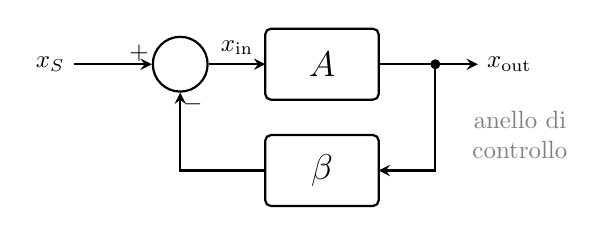
\begin{tikzpicture}[scale=0.9, transform shape]
            % Nodo sommatore
            \node[draw, circle, minimum size=22pt, thick] (sum) at (0,0) {};
            
            % Segni + e - posizionati in modo preciso e relativo vicino alle frecce
            \node[above left, inner sep=1pt] at (sum.west) {$+$};
            \node[below right, inner sep=1pt] at (sum.south) {$-$};
            
            % Ingresso x_S
            \draw[->, >=stealth, thick] (-1.5,0) node[left] {$x_S$} -- (sum.west);
            
            % Uscita sommatore verso guadagno A
            \draw[->, >=stealth, thick] (sum.east) -- (1.2,0) node[midway, above] {$x_{\mathrm{in}}$};
            \draw[thick, rounded corners=2pt] (1.2,-0.5) rectangle (2.8,0.5) node[midway, font=\Large] {$A$};
            
            % Uscita verso x_out
            \draw[->, >=stealth, thick] (2.8,0) -- (4.2,0) node[right] {$x_{\mathrm{out}}$};
            
            % Ramo di retroazione beta
            \fill (3.6,0) circle (2pt);
            \draw[->, >=stealth, thick] (3.6,0) -- (3.6,-1.5) -- (2.8,-1.5);
            \draw[thick, rounded corners=2pt] (1.2,-2.0) rectangle (2.8,-1.0) node[midway, font=\Large] {$\beta$};
            
            % Riconnessione al nodo sommatore
            \draw[->, >=stealth, thick] (1.2,-1.5) -- (0,-1.5) -- (sum.south);
            
            \node[text=gray, align=center, right] at (4.0, -1.0) {anello di\\controllo};
        \end{tikzpicture}
    \end{minipage}
    
    \caption{Schema di un amplificatore con retroazione e diagramma a blocchi dell'anello di controllo.}
\end{figure}

\noindent
La tensione differenziale $V_d$ dipende dalla tensione di uscita $V_{\mathrm{out}}$ attraverso la rete di retroazione:
\[ V_d = V_S - \frac{R_1}{R_1 + R_2} V_{\mathrm{out}} \]

\noindent
In un anello di controllo si definiscono formalmente i seguenti parametri \cite{sedra}:
\begin{itemize}[noitemsep, leftmargin=*]
    \item $A$ \textbf{(guadagno diretto)}: rapporto tra uscita e ingresso in assenza di retroazione;
    \item $\beta$ \textbf{(fattore di retroazione, \textit{feedback})}: quota del segnale di uscita rinviata al nodo sommatore.
\end{itemize}
La relazione fondamentale al nodo sommatore è:
\[
    x_{\mathrm{in}} = x_S - \beta\, x_{\mathrm{out}}
\]

\subsection*{Analisi iterativa dell'anello di controllo}

Analizzando l'evoluzione del sistema come successione discreta di stati, si ricava:
\begin{itemize}[noitemsep, leftmargin=*]
    \item $x_{\mathrm{in}}(0) = x_S, \qquad x_{\mathrm{out}}(0) = A\,x_{\mathrm{in}}(0) = A\,x_S$
    \item $x_{\mathrm{in}}(1) = x_S - \beta\,x_{\mathrm{out}}(0), \qquad x_{\mathrm{out}}(1) = A\,x_{\mathrm{in}}(1)$
    \item $\vdots$
    \item $x_{\mathrm{in}}(n) = x_S - \beta\,x_{\mathrm{out}}(n-1), \qquad x_{\mathrm{out}}(n) = A\,x_{\mathrm{in}}(n)$
\end{itemize}

\noindent
Assumendo che la successione converga, ovvero $\lim_{n \to \infty} x_{\mathrm{out}}(n) = x_{\mathrm{out}} < \infty$, in regime stazionario si ha $x_{\mathrm{out}}(n-1) \simeq x_{\mathrm{out}}(n)$. La condizione di equilibrio fornisce allora la \textbf{formula fondamentale del guadagno con retroazione}:
\[
    x_{\mathrm{out}} = A\,(x_S - \beta\,x_{\mathrm{out}})
    \qquad\Longrightarrow\qquad
    \boxed{x_{\mathrm{out}} = x_S \, \frac{A}{1 + \beta A}}
\]

\subsection*{Condizioni di stabilità dell'anello}

Se $A > 0$ e $\beta A < -1$, la successione degli stati è \textit{divergente}:
\begin{itemize}[noitemsep, leftmargin=*]
    \item \textbf{Crescente} (divergenza verso $+\infty$) se $A\,x_S > 0$.
    \item \textbf{Decrescente} (divergenza verso $-\infty$) se $A\,x_S < 0$.
\end{itemize}

\begin{osservazione}{Interpretazione fisica della divergenza}
    Il segnale esce irrimediabilmente dalla regione di linearità, portando l'amplificatore in saturazione, quando $x_{\mathrm{out}}(n) \to \infty$. Tale divergenza si manifesta anche nella condizione di equilibrio nominalmente instabile $A\,x_S = 0$, poiché il rumore termico o ambientale è sufficiente ad innescare l'anello.
\end{osservazione}

\begin{definizione}{Rumore}
    Qualsiasi perturbazione di natura aleatoria in grado di alterare il segnale di ingresso.
\end{definizione}

\noindent
In presenza di rumore, anche l'equilibrio $A\,x_S = 0$ è instabile: l'anello viene innescato da fluttuazioni termiche o ambientali. La condizione \textbf{necessaria} affinché la successione sia convergente (e il sistema sia stabile) è pertanto:
\[
    \beta A > -1
\]

\begin{osservazione}{Interpretazione geometrica della stabilità}
{\centering
    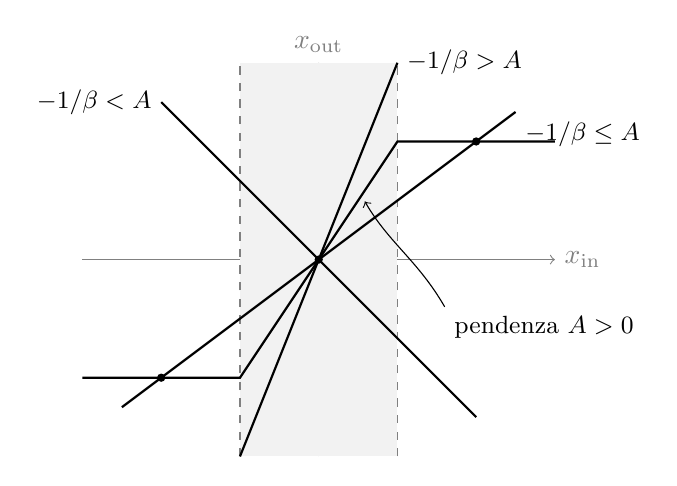
\begin{tikzpicture}[transform shape]
        % Assi
        \draw[->, gray] (-3,0) -- (3,0) node[right] {$x_{\mathrm{in}}$};
        \draw[->, gray] (0,-2.5) -- (0,2.5) node[above] {$x_{\mathrm{out}}$};
        
        % Zona lineare
        \fill[gray!10] (-1,-2.5) rectangle (1,2.5);
        \draw[gray, dashed] (-1,-2.5) -- (-1,2.5);
        \draw[gray, dashed] (1,-2.5) -- (1,2.5);
        
        % Caratteristica dell'amplificatore (pendenza A > 0)
        \draw[thick] (-3,-1.5) -- (-1,-1.5) -- (1,1.5) -- (3,1.5);
        \node[anchor=north west] at (1.6, -0.6) {\small pendenza $A>0$};
        \draw[->, shorten >=2pt] (1.6, -0.6) to[out=120, in=300] (0.55, 0.8);
        
        % Rette di carico (pendenza $-1/\beta$)
        \draw[thick] (-2, 2) -- (2, -2);
        \node[anchor=east] at (-2, 2) {\small $-1/\beta < A$};
        
        \draw[thick] (-2.5, -1.875) -- (2.5, 1.875);
        \node[anchor=north west] at (2.5, 1.875) {\small $-1/\beta \le A$};
        
        \draw[thick] (-1, -2.5) -- (1, 2.5);
        \node[anchor=west] at (1, 2.5) {\small $-1/\beta > A$};
        
        % Punti di intersezione
        \fill (0,0) circle (1.5pt);
        \fill (2, 1.5) circle (1.5pt); 
        \fill (-2, -1.5) circle (1.5pt); 
    \end{tikzpicture}\par}

\medskip
Le due equazioni da intersecare graficamente sono:
\begin{itemize}[noitemsep, leftmargin=*]
    \item $x_{\mathrm{out}} = A\,x_{\mathrm{in}}$: caratteristica dell'amplificatore (pendenza $A$).
    \item $x_{\mathrm{out}} = x_S/\beta - x_{\mathrm{in}}/\beta$: retta di carico (pendenza $-1/\beta$).
\end{itemize}

\medskip
\textbf{Classificazione delle intersezioni (per $A>0$):}
\begin{itemize}[noitemsep, leftmargin=*]
    \item $\beta > 0,\; \beta A \le -1$: condizione impossibile ($\beta > 0$ e $\beta A \le -1$ sono incompatibili per $A > 0$) $\Rightarrow$ \textbf{nessuna soluzione reale}.
    \item $\beta < 0,\; \beta A \le -1 \Rightarrow \beta \le -1/A < 0 \Rightarrow -1/\beta \le A$: \textbf{1 o 3 intersezioni} (con punti in saturazione).
    \item $\beta > 0,\; \beta A > -1 \Rightarrow \beta > 0 > -1/A \Rightarrow -1/\beta < A$: \textbf{1 intersezione} (in regione lineare o di saturazione).
    \item $\beta < 0,\; \beta A > -1 \Rightarrow 0 > \beta > -1/A \Rightarrow -1/\beta > A$: \textbf{1 intersezione} (in regione lineare o di saturazione).
\end{itemize}

\smallskip
\begin{note}La pendenza della retta di carico è $-1/\beta$; se $\beta < 0$ la pendenza è positiva, il che riflette la natura del feedback positivo.\end{note}
\end{osservazione}

\section{Applicazione ai circuiti con l'Op-Amp}

\subsection*{Caso ideale e condizione per il feedback negativo}

Nel caso ideale in cui il guadagno differenziale sia infinito ($A_d \to +\infty$), la condizione di stabilità dell'anello $\beta > -1/A_d$ diviene semplicemente:
\[
    \beta > -\frac{1}{A_d} \xrightarrow{A_d \to +\infty} 0
\]
Geometricamente, ciò equivale a richiedere che la retta di carico abbia \textit{pendenza negativa} (poiché $-1/\beta < 0$ quando $\beta > 0$). Si configura dunque un sistema con \textbf{feedback negativo}, in cui il segnale al nodo sommatore è:
\[
    x_{\mathrm{in}} = x_S - |\beta|\, x_{\mathrm{out}}
\]
Al contrario, quando $\beta < 0$ la retroazione è \textit{positiva} e la pendenza della retta di carico è positiva: il sistema risulta instabile in zona lineare e si porta necessariamente in saturazione.

\medskip
\noindent
Per chiarire il ruolo del segno di $\beta$, analizziamo due configurazioni fondamentali dell'amplificatore operazionale.

\begin{figure}[H]
    \centering
    \begin{minipage}[t]{0.48\textwidth}
        \centering
        \begin{circuitikz}[american, thick, scale=0.85]
            % opamp specchiato: il terminale + in alto, - in basso
            \draw (0,0) node[op amp, yscale=-1] (opamp) {};
            
            % Ingresso non invertente (+) in alto
            \draw (opamp.+) to[short, -o] ++(-1.5, 0) node[left] {$V_S$};
            
            % Partitore di retroazione sul terminale invertente (-) in basso
            \draw (opamp.-) -- ++(0, -1) coordinate(div_node);
            \draw (div_node) to[R, l_=$R_1$] ++(0, -1.8) node[ground]{};
            \draw (div_node) to[R, l_=$R_2$] (div_node -| opamp.out) -- (opamp.out);
            
            % Uscita
            \draw (opamp.out) to[short, *-o] ++(1, 0) node[right] {$V_{out}$};
        \end{circuitikz}
        \par\smallskip{\small \textbf{(a)} Amplificatore non invertente: feedback \textbf{negativo} ($\beta > 0$).}
    \end{minipage}%
    \hfill
    \begin{minipage}[t]{0.48\textwidth}
        \centering
        \begin{circuitikz}[american, thick, scale=0.85]
            % opamp standard: - in alto, + in basso
            \draw (0,0) node[op amp] (opamp) {};
            
            % Ingresso invertente (-) in alto
            \draw (opamp.-) to[short, -o] ++(-1.5, 0) node[left] {$V_S$};
            
            % Partitore di retroazione sul terminale non invertente (+) in basso
            \draw (opamp.+) -- ++(0, -1) coordinate(div_node);
            \draw (div_node) to[R, l_=$R_1$] ++(0, -1.8) node[ground]{};
            \draw (div_node) to[R, l_=$R_2$] (div_node -| opamp.out) -- (opamp.out);
            
            % Uscita
            \draw (opamp.out) to[short, *-o] ++(1, 0) node[right] {$V_{out}$};
        \end{circuitikz}
        \par\smallskip{\small \textbf{(b)} Trigger di Schmitt invertente: feedback \textbf{positivo} ($\beta < 0$).}
    \end{minipage}
\end{figure}

\noindent
\textbf{Esempio 1: Amplificatore non invertente (feedback negativo)} \\
Il partitore formato da $R_1$ ed $R_2$ riporta una frazione dell'uscita al terminale invertente ($V_-$). La tensione differenziale vale:
\[
    V_d = V_+ - V_- = V_S - \frac{R_1}{R_1 + R_2}\,V_{out}
\]
Il fattore di retroazione è pertanto $\beta = \dfrac{R_1}{R_1 + R_2} > 0$, e il feedback si definisce \textbf{negativo}: l'uscita viene sottratta dall'ingresso, stabilizzando il sistema.

\medskip
\noindent
\textbf{Esempio 2: Trigger di Schmitt invertente (feedback positivo)} \\
In questa configurazione il partitore $R_1$--$R_2$ riporta una frazione dell'uscita al terminale non invertente ($V_+$), mentre il segnale $V_S$ è applicato al terminale invertente. La tensione differenziale diviene:
\[
    V_d = V_+ - V_- = \frac{R_1}{R_1 + R_2}\,V_{out} - V_S
    = -\!\left(V_S - \frac{R_1}{R_1 + R_2}\,V_{out}\right)
\]
In questo caso il segno globale della retroazione è invertito: l'uscita viene sommata all'ingresso. Scrivendo $V_d = x_S - \beta V_{out}$ con $x_S = -V_S$, si riconosce un fattore $\beta = -\frac{R_1}{R_1+R_2} < 0$, e il feedback si definisce \textbf{positivo}.

\begin{osservazione}{Non linearità del feedback positivo}
    Un sistema con feedback positivo è intrinsecamente instabile nella regione lineare dell'amplificatore: qualunque perturbazione (incluso il rumore termico) viene amplificata ad ogni ciclo dell'anello, provocando una crescita esponenziale del segnale fino alla saturazione. Il comportamento risultante (con un'uscita che commuta tra i due livelli di saturazione $\pm V_{\mathrm{sat}}$) è quello di un comparatore con isteresi (circuito di Schmitt trigger), dal carattere spiccatamente non lineare. Per questo motivo, nelle applicazioni lineari si impiega esclusivamente il feedback negativo.
\end{osservazione}

\subsection*{Proprietà del feedback negativo: desensibilizzazione del guadagno}

Uno dei vantaggi fondamentali dell'anello di retroazione negativa è la ridotta sensibilità del guadagno complessivo alle fluttuazioni dei parametri costruttivi dei dispositivi attivi, i quali sono intrinsecamente soggetti a grande indeterminazione: $A \pm \sigma(A)$, con $\sigma(A)$ elevata.

\medskip
\noindent
L'idea è la seguente: \emph{modificare il circuito} (aggiungendo la retroazione) in modo da \emph{rendere il guadagno indipendente} dai parametri costruttivi che sono affetti da grande incertezza, e farlo dipendere esclusivamente da componenti passivi (resistori, la cui tolleranza è molto più stretta). Siano:
\begin{itemize}[noitemsep, leftmargin=*]
    \item $A = \left.\dfrac{V_{out}}{V_S}\right|_{\beta=0}$: guadagno \textit{open-loop} (senza retroazione);
    \item $A_f = \left.\dfrac{V_{out}}{V_S}\right|_{\beta>0} = \dfrac{A}{1 + \beta A} = A\,(1 + \beta A)^{-1}$: guadagno \textit{closed-loop} (con retroazione applicata).
\end{itemize}

\noindent
Calcoliamo ora la sensibilità del guadagno $A_f$ rispetto a variazioni di $A$. La derivata parziale è:
\[
    \frac{\partial A_f}{\partial A} = \frac{\partial}{\partial A}\!\left(\frac{A}{1 + \beta A}\right) = \frac{(1+\beta A) - A\,\beta}{(1+\beta A)^2} = \frac{1}{(1 + \beta A)^2}
\]
L'incertezza assoluta sul guadagno ad anello chiuso vale pertanto:
\[
    \sigma(A_f) = \left|\frac{\partial A_f}{\partial A}\right| \sigma(A) = \frac{\sigma(A)}{(1 + \beta A)^2}
\]
Possiamo riscriverla evidenziando l'incertezza relativa open-loop:
\[
    \sigma(A_f) = \frac{A}{(1 + \beta A)^2} \cdot \frac{\sigma(A)}{A}
    = \underbrace{\frac{A}{1 + \beta A}}_{= A_f} \cdot \underbrace{\frac{1}{1 + \beta A}}_{\text{desensibilizzazione}} \cdot \frac{\sigma(A)}{A}
\]
Dividendo per $A_f$ si ottiene l'\textbf{incertezza relativa} del guadagno con retroazione:
\[
    \boxed{\;\sigma_{\mathrm{rel}}(A_f) = \frac{\sigma(A_f)}{A_f} = \frac{1}{1 + \beta A}\;\sigma_{\mathrm{rel}}(A)\;}
\]
Il termine $\dfrac{1}{1 + \beta A}$ è il \textbf{fattore di desensibilizzazione del guadagno}: per $\beta A \gg 1$ l'incertezza relativa viene drasticamente ridotta.

\medskip
\begin{osservazione}{Approssimazione del guadagno ad anello chiuso}
    Anche se il guadagno diretto $A$ è fortemente indeterminato, l'unica conseguenza è un modesto scostamento dal valore ideale $A_f \approx 1/\beta$. Il grado di accuratezza di $A_f$ è stabilito principalmente dalla tolleranza dei componenti passivi che definiscono $\beta$, e non dalle fluttuazioni di $A$.
\end{osservazione}

\subsection*{Proprietà del feedback negativo: adattamento delle impedenze}

Oltre a stabilizzare il guadagno, la retroazione modifica le impedenze di ingresso e di uscita del circuito --- indicate rispettivamente con $Z_{in,F}$ e $Z_{out,F}$ (il pedice $F$ sta per \textit{Feedback}) --- rispetto a quelle dell'amplificatore privo di reazione ($Z_{in}$ e $Z_{out}$).

\begin{figure}[H]
    \centering
    \begin{circuitikz}[american, thick, scale=1.0]
        
        % Amplificatore (Riquadro superiore)
        \draw[fill=black!5, rounded corners] (0, 0) rectangle (6, 3);
        \node[above] at (3, 3) {\textbf{Amplificatore Base ($A$)}};
        
        % Componenti interni all'amplificatore
        \draw (0, 2.2) -- (1, 2.2) to[R, l=$Z_{in}$] (1, 0.8) -- (0, 0.8);
        \draw (6, 2.2) -- (5, 2.2) to[R, l_=$Z_{out}$] (3.5, 2.2) to[cV, l=$A V_{in}$] (3.5, 0.8) -- (6, 0.8);
        
        % Rete di retroazione (Riquadro inferiore)
        \draw[fill=black!5, rounded corners] (2, -3) rectangle (4, -1);
        \node at (3, -2) {\Large $\beta$};
        
        % Maglia di ingresso (Connessione in Serie)
        \draw (-3, -1.5) to[sV, l=$V_S$, i=$I_S$] (-3, 2.2) -- (0, 2.2);
        \draw (0, 0.8) -- (0, -1.5) -- (2, -1.5); % Da Zin verso l'ingresso + di beta
        \draw (-3, -1.5) -- (-3, -2.5) -- (2, -2.5); % Dal generatore verso l'ingresso - di beta
        
        % Maglia di uscita (Connessione in Parallelo)
        \draw (6, 2.2) -- (7.5, 2.2) to[short, -o] (8.5, 2.2);
        \draw (6, 0.8) -- (7.5, 0.8) to[short, -o] (8.5, 0.8);
        
        % Derivazione dell'uscita verso beta
        \draw (6.5, 2.2) node[circ]{} -- (6.5, -1.5) -- (4, -1.5); % Dal terminale alto dell'uscita a beta
        \draw (7.0, 0.8) node[circ]{} -- (7.0, -2.5) -- (4, -2.5); % Dal terminale basso dell'uscita a beta
        
        % Etichette e correnti esterne
        \draw[decorate,decoration={brace,amplitude=6pt}] (-0.2,0.8) -- (-0.2,2.2) node[midway,left=8pt] {$V_{in}$};
        
        \draw[decorate,decoration={brace,amplitude=6pt}] (8.7,2.2) -- (8.7,0.8) node[midway,right=8pt] {$V_{out}$};
        \node[right, align=left] at (9.8, 1.5) {sul carico $R_L$};
        
        \draw[->, >=stealth] (7.8, 2.4) -- (8.5, 2.4) node[above] {$I_{out}$};
        
    \end{circuitikz}
    \caption{Modello dell'amplificatore con retroazione (topologia tensione-tensione): campionamento in parallelo all'uscita, reinserzione in serie all'ingresso.}
\end{figure}

\noindent
Per la \textbf{topologia tensione-tensione} (campionamento in parallelo sull'uscita, reinserzione in serie all'ingresso), le impedenze si modificano come segue.

\medskip
\noindent
\textbf{Impedenza d'ingresso reazionata.} L'impedenza dell'amplificatore senza retroazione è $Z_{in} = V_{in}/I_S$. Con la retroazione, la tensione ai capi dell'ingresso del sorgente è $V_S = V_{in} + \beta V_{out}$. Poiché $V_{out} = A V_{in}$:
\[
    V_S = V_{in}(1 + \beta A) \qquad \Longrightarrow \qquad
    Z_{in,F} = \frac{V_S}{I_S} = \frac{V_{in}(1 + \beta A)}{I_S} = Z_{in}\,(1 + \beta A) \gg Z_{in} \quad \text{per } \beta A \gg 1
\]

\medskip
\noindent
\textbf{Impedenza d'uscita reazionata.} Per calcolare $Z_{out,F}$ si applica un generatore di test all'uscita con sorgente spenta ($V_S = 0$):
\[
    Z_{out,F} = \frac{V_{out}}{I_{out}}
\]
Con $V_S = 0$ la rete di retroazione impone $V_{in} = -\beta V_{out}$, quindi il generatore interno vale $A V_{in} = -\beta A\, V_{out}$. La corrente entrante nell'uscita attraversa $Z_{out}$:
\[
    I_{out} = \frac{V_{out} - A V_{in}}{Z_{out}} = \frac{V_{out}(1 + \beta A)}{Z_{out}}
    \qquad\Longrightarrow\qquad
    Z_{out,F} = \frac{Z_{out}}{1 + \beta A} \ll Z_{out} \quad \text{per } \beta A \gg 1
\]

\medskip
\noindent
In sintesi, la retroazione tensione-tensione avvicina il circuito al comportamento di un \textbf{generatore di tensione ideale pilotato in tensione}: l'impedenza d'ingresso tende a infinito ($Z_{in,F} \to \infty$) e quella d'uscita tende a zero ($Z_{out,F} \to 0$).

\subsection*{Esempio: amplificatore non invertente con Op-Amp ideale}

Verifichiamo le proprietà generali sull'amplificatore non invertente con $A_d \to \infty$ (caso limite ideale), in cui valgono il Cortocircuito Virtuale (CCV) e la condizione $Z_{in} \to \infty$.

\begin{figure}[H]
    \centering
    \begin{circuitikz}[american, thick, scale=0.85, transform shape]
        % Triangolo Op-Amp molto ampio
        \draw[fill=black!5, thick] (0, 5) -- (10, 0) -- (0, -5) -- cycle;
        
        % Etichette morsetti - e +
        \node[above] at (0.5, 2) {\Large $-$};
        \node[below] at (0.5, -2) {\Large $+$};
        
        % Connessione dai morsetti d'ingresso a Zin
        \draw (0, 2) -- (2.5, 2);
        \draw (0, -2) -- (2.5, -2);
        
        % Zin
        \draw (2.5, -2) to[R, l=$Z_{in}$] (2.5, 2);
        
        % Tensione differenziale Vd (con graffa)
        \draw[decorate,decoration={brace,mirror,amplitude=6pt}] (3.3, -1.8) -- (3.3, 1.8) node[midway, right=10pt] {$V_d$};
        \node[font=\small] at (3.3, 2) {$-$};
        \node[font=\small] at (3.3, -2) {$+$};
        
        % Generatore dipendente e Zout all'interno
        \draw (5, -1.5) node[ground]{} to[cV, l_=$A_d V_d$] (5, 0) to[R, l=$Z_{out}$] (10, 0);
        
        % Connessioni esterne: Ingresso invertente (-) e R1 a massa
        \draw (0, 2) -- (-2.5, 2) coordinate(in_neg);
        \draw (in_neg) to[R, l_=$R_1$] (-2.5, 0) node[ground]{};
        
        % Retroazione R2
        \draw (in_neg) -- (-2.5, 6) to[R, l=$R_2$] (11.5, 6) -- (11.5, 0);
        
        % Ingresso non invertente (+) e V_S
        \draw (0, -2) to[short, -o] (-3.0, -2) node[left] {$V_S$};
        \draw[->, >=stealth] (-2.5, -1.7) -- (-0.5, -1.7) node[midway, above] {$I_S$};
        
        % Uscita e Carico RL
        \draw (10, 0) -- (11.5, 0) coordinate(out_node);
        \draw (out_node) node[circ]{} to[short, -o] (13.5, 0) node[right] {$V_{out}$};
        \draw (out_node) to[R, l=$R_L$] (11.5, -4) node[ground]{};
        
        % Corrente di uscita
        \draw[->, >=stealth] (10.3, 0.4) -- (11.2, 0.4) node[midway, above] {$I_{out}$};
        
    \end{circuitikz}
    \caption{Amplificatore non invertente con retroazione: schema completo con impedenza d'uscita $Z_{out}$ e carico $R_L$. Nel limite ideale $A_d \to \infty$ si applicano le proprietà del CCV.}
\end{figure}

\noindent
Con $A_d \to \infty$ e il Cortocircuito Virtuale ($V_+ = V_-$, $I_S = 0$):

\begin{itemize}[noitemsep, leftmargin=*]
    \item \textbf{Impedenza d'ingresso:} $Z_{in,F} = \dfrac{V_S}{I_S} \to \infty$, poiché nel CCV la corrente assorbita dall'ingresso è nulla ($I_S = 0$).
    
    \item \textbf{Guadagno:} dal partitore di tensione al morsetto invertente si ha $V_- = \dfrac{R_1}{R_2 + R_1}\,V_{out}$. Imponendo il CCV ($V_- = V_+ = V_S$):
    \[
        V_S = \frac{R_1}{R_2 + R_1}\,V_{out} \qquad \Longrightarrow \qquad V_{out} = \left(1 + \frac{R_2}{R_1}\right) V_S
    \]
    
    \item \textbf{Impedenza d'uscita:} $Z_{out,F} \to 0$, poiché la tensione d'uscita è forzata dal CCV al valore $V_{out} = (1 + R_2/R_1)\,V_S$ \emph{indipendentemente} dal carico: variando $R_L$ cambia la corrente $I_{out}$ ma non $V_{out}$, cioè $\Delta V_{out}/\Delta I_{out} = 0$. L'uscita si comporta quindi come un generatore di tensione ideale, con impedenza d'uscita nulla (coerente con $Z_{out,F} = Z_{out}/(1+\beta A_d) \to 0$).
\end{itemize}

\medskip
\noindent
\begin{note}Con le altre topologie si ottengono adattamenti diversi. Ad esempio, con la topologia corrente-corrente (campionamento in serie sull'uscita, reinserzione in parallelo all'ingresso), adatta a una sorgente di corrente, la retroazione \emph{riduce} l'impedenza d'ingresso e \emph{aumenta} quella d'uscita: $Z_{in,F} = Z_{in}/(1+\beta A)$, $Z_{out,F} = Z_{out}(1+\beta A)$. Il circuito si avvicina così a un amplificatore di corrente ideale ($Z_{in} \to 0$, $Z_{out} \to \infty$), come l'amplificatore invertente di corrente visto sopra.\end{note}

\section*{Riepilogo del Capitolo}

\begin{important}
Il \textbf{Cortocircuito Virtuale} (conseguenza del Teorema di Miller applicato al limite $A_d \to \infty$) rende immediato il calcolo del guadagno di qualunque configurazione con operazionale, mentre la teoria della retroazione ($x_{out} = x_S \, A/(1+\beta A)$) ne spiega la stabilità, la desensibilizzazione del guadagno e l'adattamento delle impedenze.
\end{important}

\begin{note}
\textbf{Formule fondamentali:}
\begin{itemize}
    \item \textbf{Cortocircuito Virtuale (CCV):} $V_+ = V_-$, correnti nulle nei terminali d'ingresso (\cref{sec:ccv}).
    \item \textbf{Invertente / Non invertente:} $A_V = -R_2/R_1$ \quad / \quad $A_V = 1+R_2/R_1$.
    \item \textbf{Guadagno con retroazione:} $x_{out} = x_S \dfrac{A}{1+\beta A}$; condizione di stabilità $\beta A > -1$.
    \item \textbf{Desensibilizzazione del guadagno:} $\sigma_{rel}(A_f) = \dfrac{1}{1+\beta A}\,\sigma_{rel}(A)$.
    \item \textbf{Impedenze reazionate (topologia tensione-tensione):} $Z_{in,F} = Z_{in}(1+\beta A)$, $\; Z_{out,F} = Z_{out}/(1+\beta A)$.
    \item \textbf{Teorema di Miller} (richiamato dal \cref{sec:miller-bjt}): $Z_{in} = Z/(1-A)$, $\; Z_{out} = \dfrac{A}{A-1}Z$.
\end{itemize}
\end{note}

